\chapter{工业应用}
\section{神经网络部署}
% 
第三、四部分中多次提到的MATLAB Coder就是一个可以将MATLAB源码转化为性能更高的C代码,以下是工程化部署的编译链以及几种主流编程语言编写本项目中的FFT算法的Benchmark。\par
\begin{figure}[htp]
    \centering
    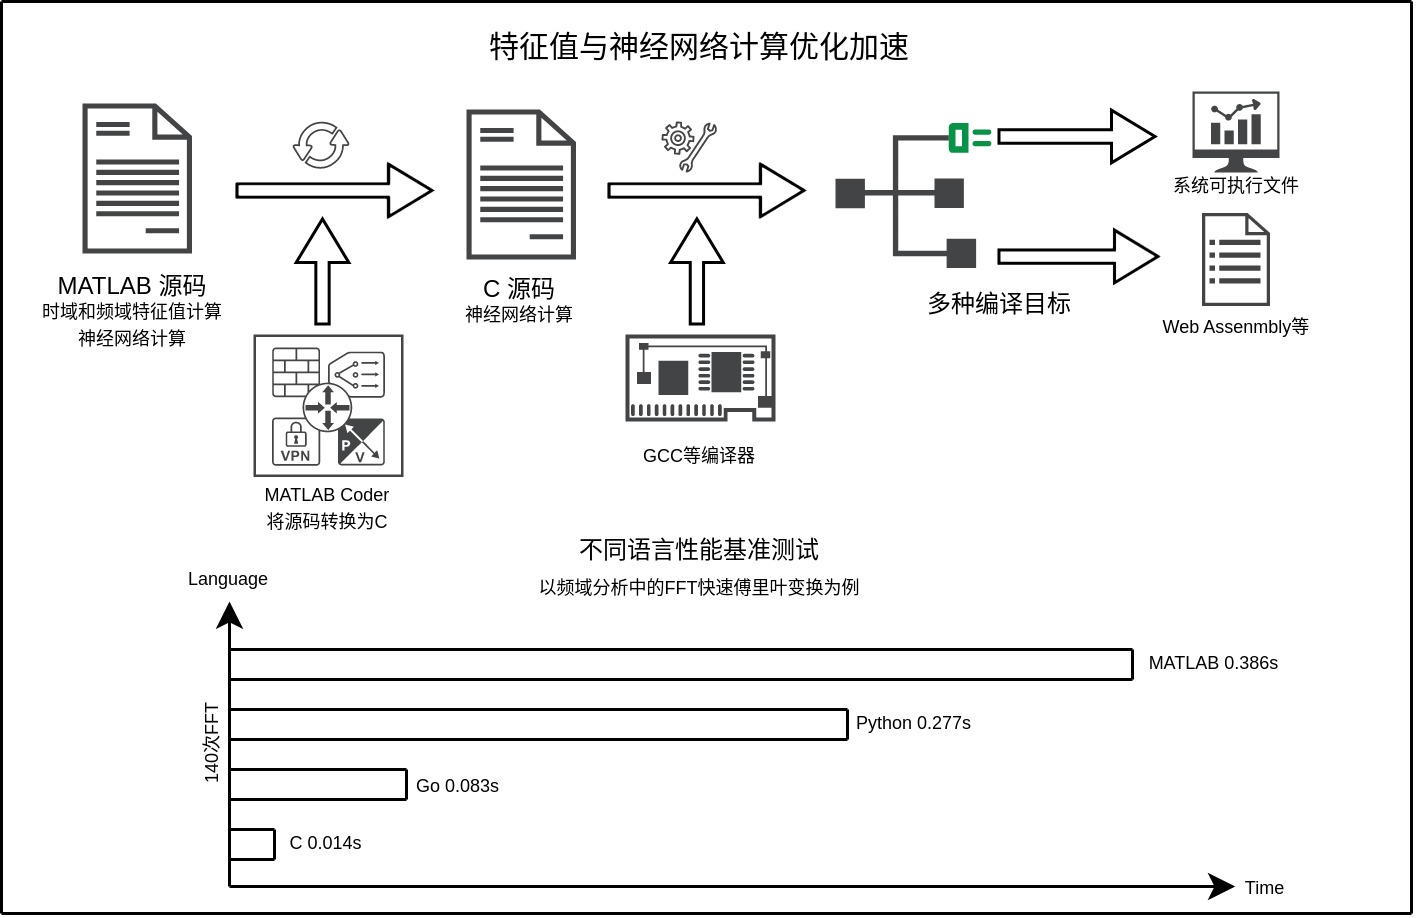
\includegraphics[width=14cm]{Chapter5/compile_chain.jpg}
    \caption{机床传感器信号图像}
\end{figure}
% 
% 
% 
\section{刀具备件管理系统的设计与搭建}
为保证工业企业生产加工的连续性、高效率,需要对数控机床上的刀具进行必要的备件储备。若刀具备件过少,会影响零件加工的连续性,降低工业企业的生产效率;若刀具备件过多,会使超额刀具长期存放,造成不必要的仓储管理费用,且存放时间过长会造成腐蚀,增加成本。因此,确定合理的刀具备件储备量可有效满足零件加工的需要,提高工业企业的生产效率,增加经济收益。\par
未来,我们将设计搭建OpenIE刀具备件管理系统,设计可以实现确定刀具备件量、数字化记录刀具备件数据、并实现相关数据统计分析等功能的软件系统,如下图所示。\par
\begin{figure}[htp]
    \centering
    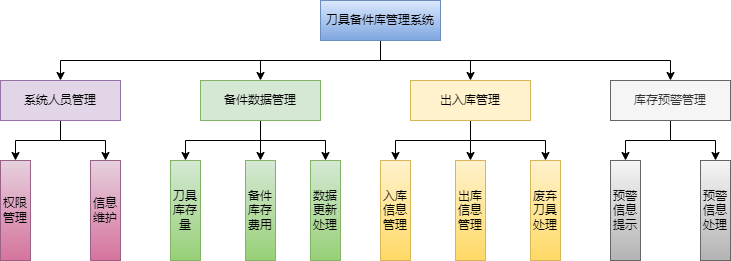
\includegraphics[width=12cm]{Chapter5/刀具备件库管理系统的设计.png}
    \caption{刀具备件库管理系统的设计}
\end{figure}
利用刀具备件库管理系统可线上实现系统人员管理、备件数据管理、出入库管理、库存预警管理。在每一个模块下,可实现对刀具备件更细化的管理:\par
(1)在系统人员管理中,可控制管理人员的操作权限与信息维护;
(2)备件数据管理中,可对查询刀具库存量、备件库存费用,并进行相关数据的更新;
(3)出入库管理中,可对刀具的入库、出库信息进行管理,并处理废弃刀具;
(4)库存预警管理中,可以及时发送刀具磨损的预警信息,同时,管理人员可对预警信息进行处理。
以上,即为OpenIE刀具备件库管理系统的设计与搭建。
% \section{}
% \subsection{}
% \begin{figure}[htp]
%     \centering
%     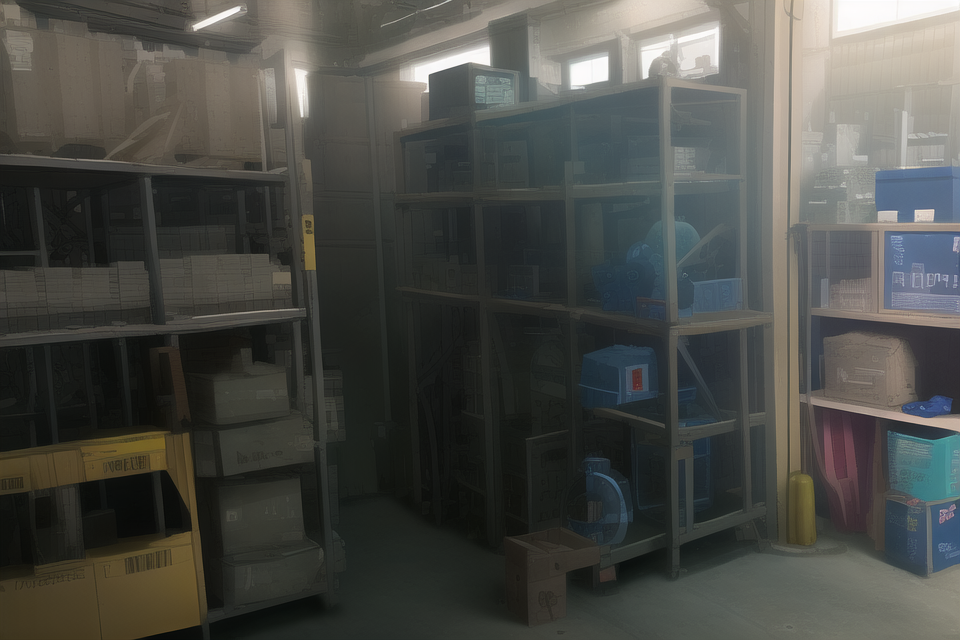
\includegraphics[width=12cm]{Chapter5/store.png}
%     \caption{工厂备件库}
% \end{figure}
% 
\newpage
\section{边缘计算硬件设备部署}
\begin{figure}[htp]
    \centering
    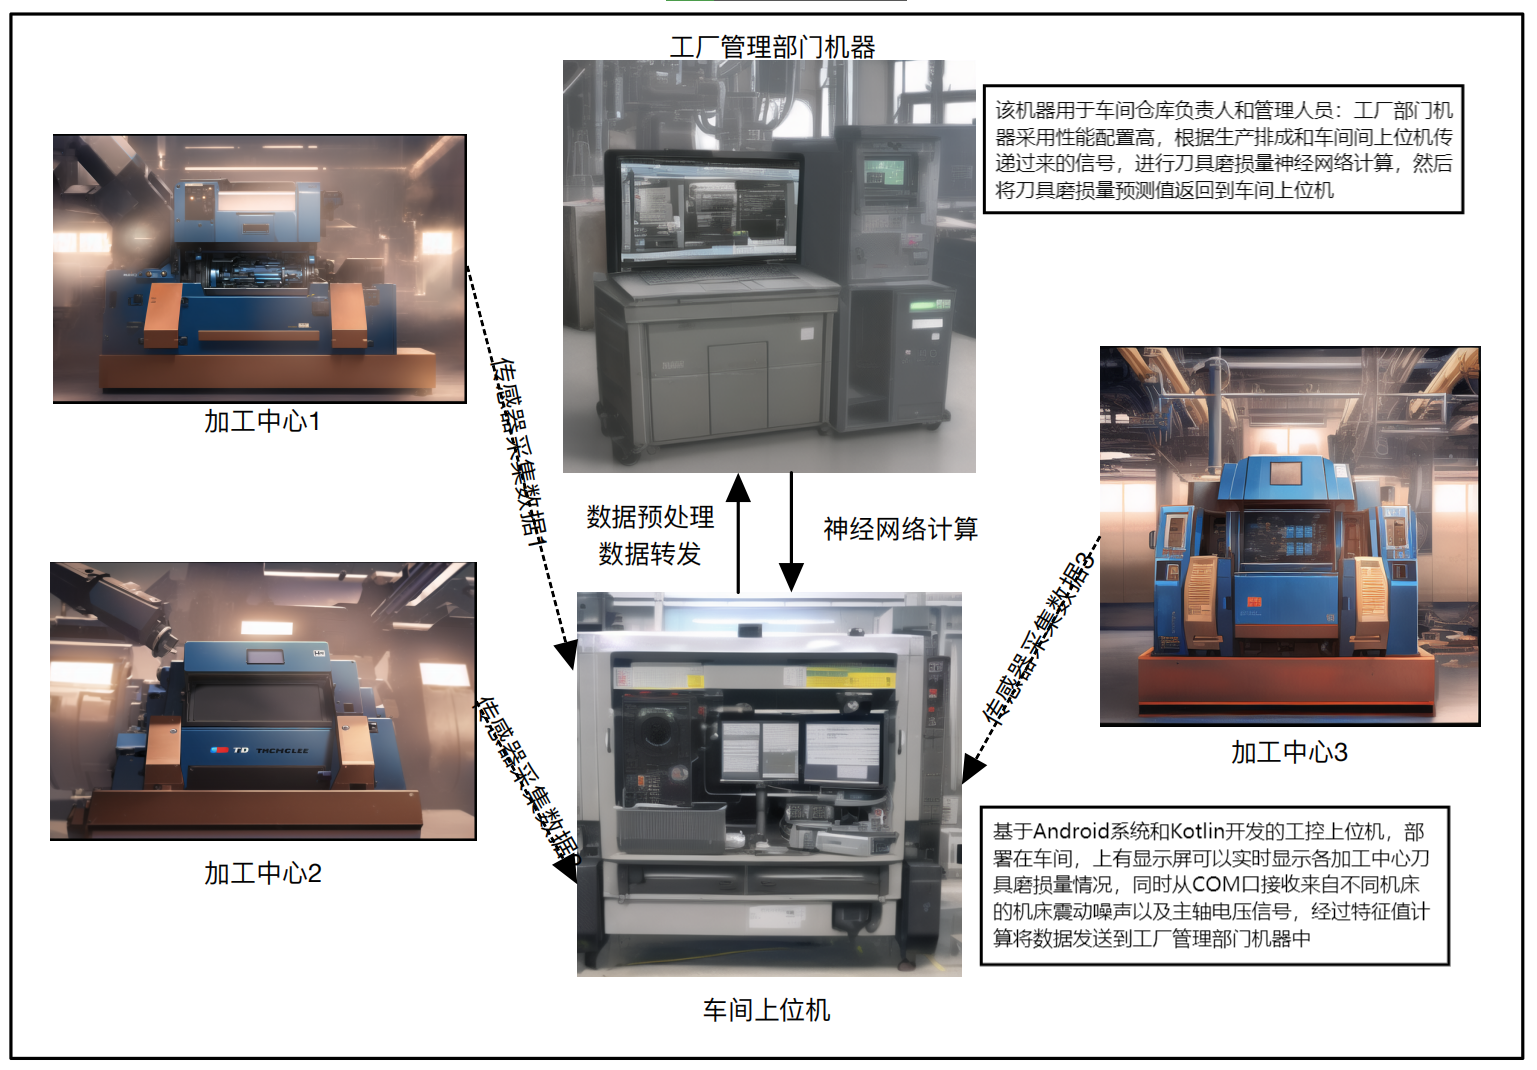
\includegraphics[width=14cm]{Chapter5/network.png}
    \caption{边缘计算硬件设备}
\end{figure}
我们设计的刀具退化预测边缘计算架构由四层组成,它们分别是:由加工中心组成的设备层(产生信号),由PLC或是单片机组成的传输层(将设备层获取到的传感器信号传递给边缘计算层),由边缘设备(工控机或是计算机浏览器等)组成的边缘计算层(负责计算信号特征值、绘制信号图像、传递特征值给云端设备以及显示云端设备返回的刀具退化程度),由云服务器或是高性能计算机组成的云计算层(将获取到的机床特征值进行神经网络计算,预测刀具退化程度并把该数据返回给边缘计算层)。\par
图5.3中显示车间上位机就是处于边缘计算层,负责把设备层中的几个加工中心数据计算特征值,并把特征值发送给云端的服务器进行神经网络计算。\par
% 
\newpage
\section{工业组件化制造执行系统}
% \begin{figure}[htp]
%     \centering
%     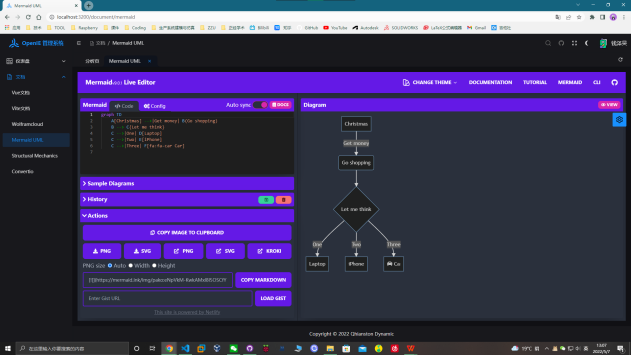
\includegraphics[width=6cm]{Chapter4/mes.png}
%     \caption{OpenIE制造执行系统}
% \end{figure}
% 
\subsection{信号可视化程序}
使用 \href{https://streamlit.io/}{streamlit} 这个Python后端框架开发进行数据可视化,我们在设计OpenIE系统的时候参考了当下互联网企业的微服务框架,即组建化开发,把一个大型项目拆分成一个个小的项目,这样使得代码更容易被维护,我们程序中人机交互部分主要采用的是HTML网页,这样做的好处是非常容易将各模块嵌入到其他网页或是APP中。\par
本部分已经在Gitee中开源,\href{https://gitee.com/qian_zehao/OpenIE}{链接跳转https://gitee.com/qian\_zehao/OpenIE} \par
\begin{figure}[htbp]
% \centering
\begin{minipage}[t]{0.48\textwidth}
\centering
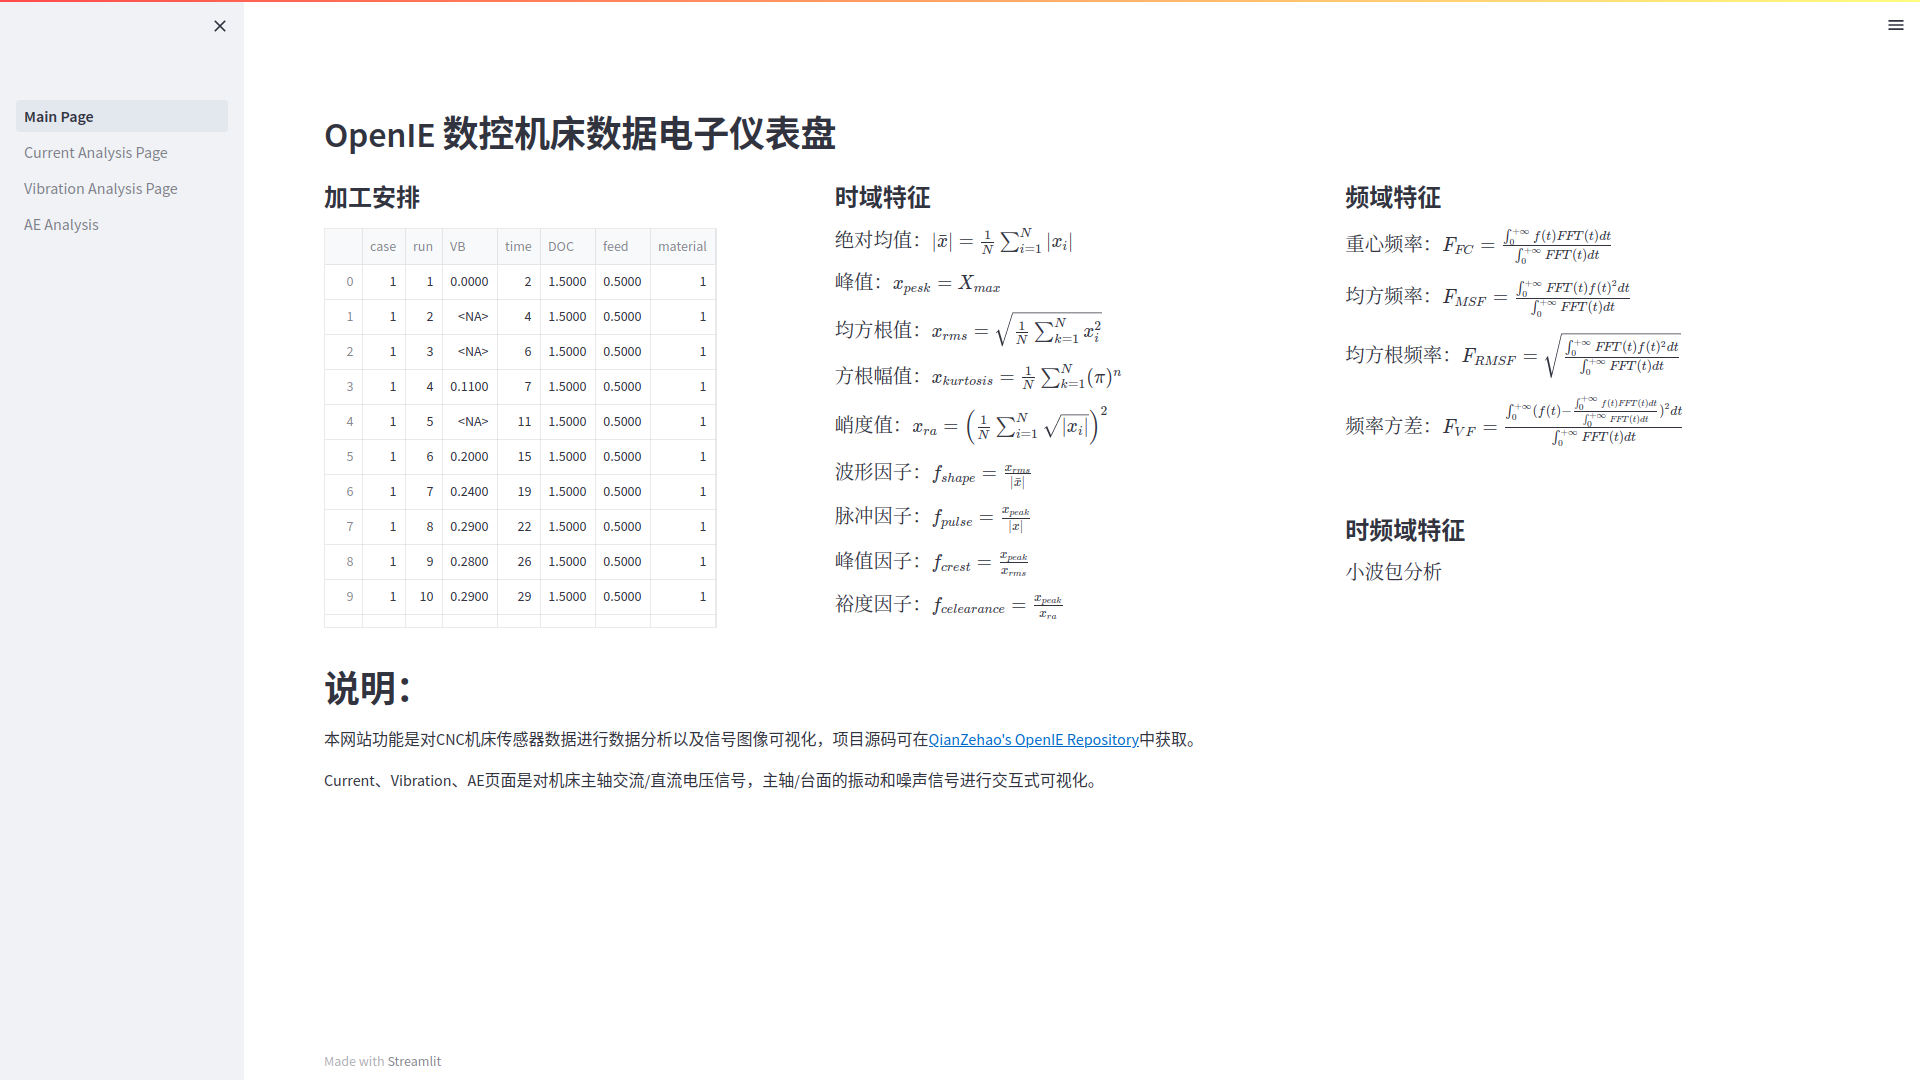
\includegraphics[width=6cm]{Chapter5/mainpage.jpeg}
% \label{fig_22}
\caption{数据分析主页}
\end{minipage}
\begin{minipage}[t]{0.48\textwidth}
\centering
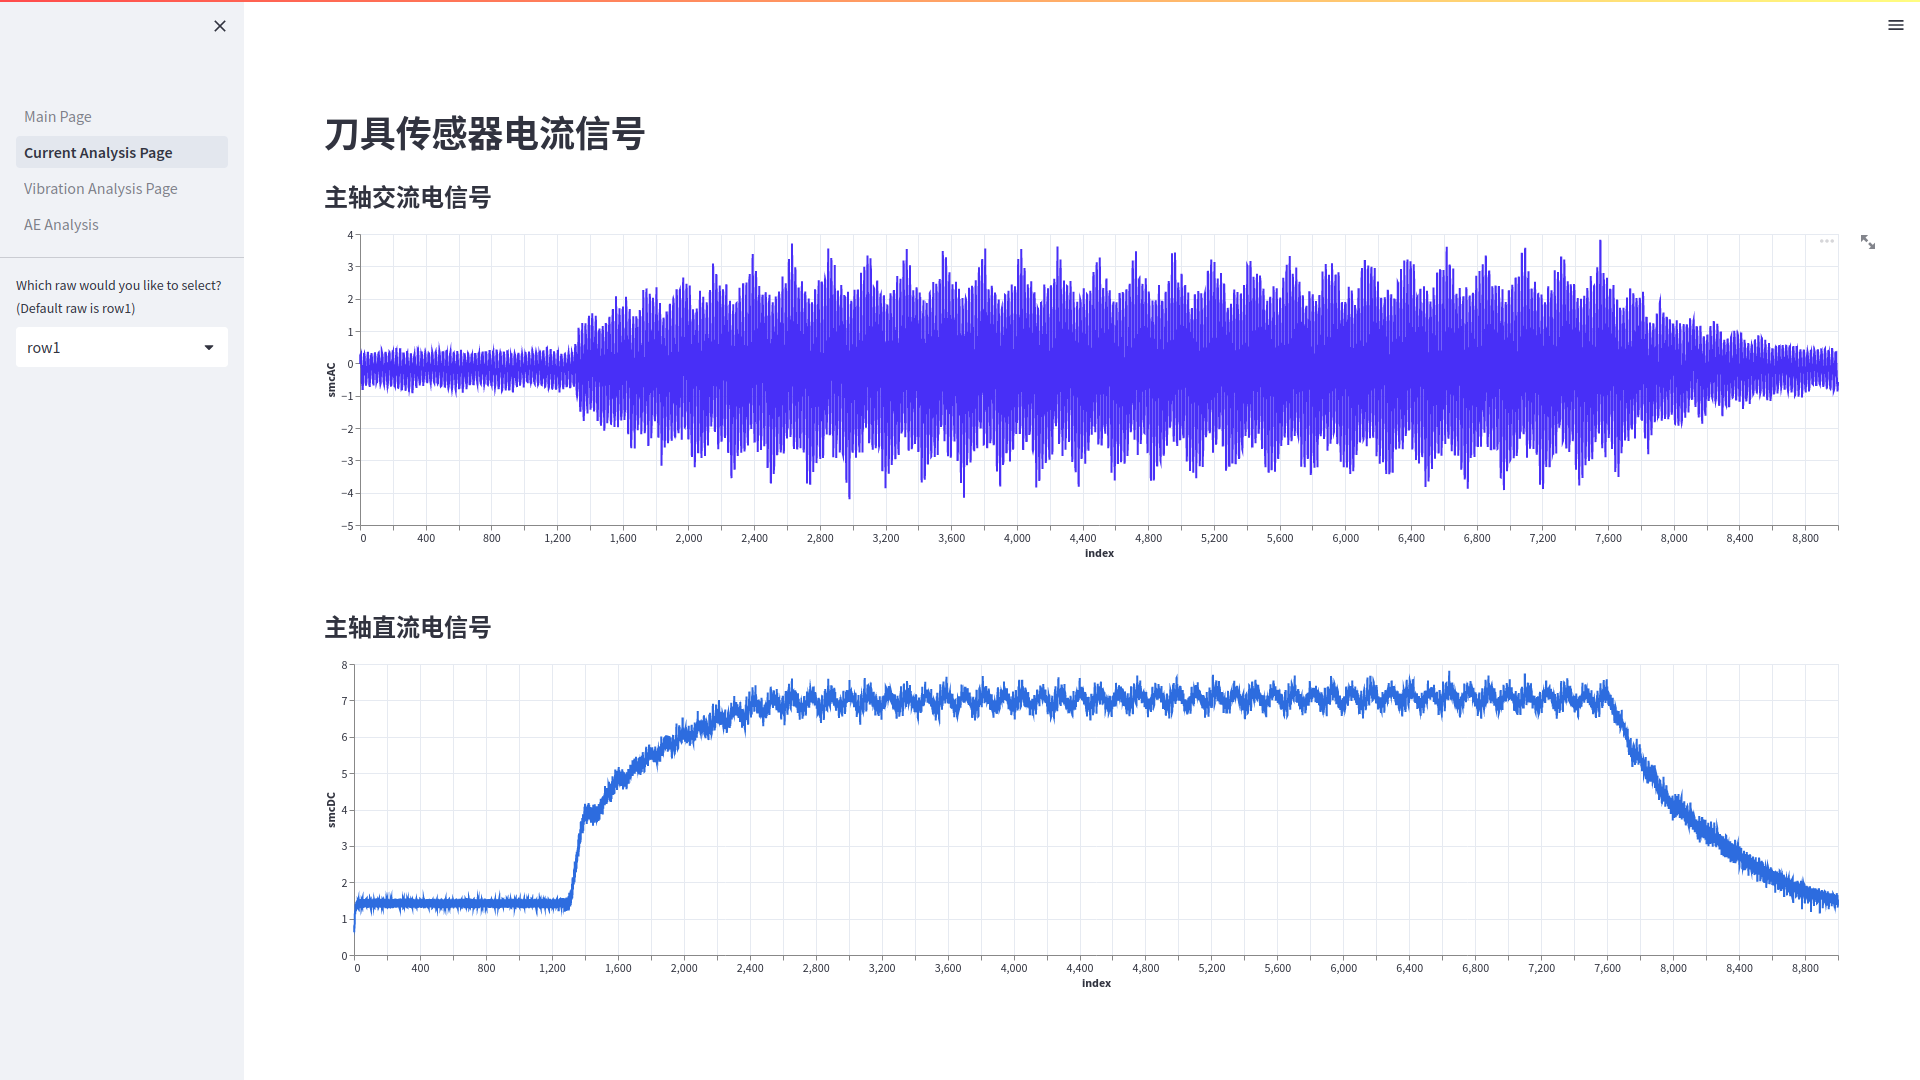
\includegraphics[width=6cm]{Chapter5/current.jpeg}
  \caption{电压数据分析}
% \label{fig_23}
\end{minipage}
\end{figure}
% 
% 
\begin{figure}[htbp]
% \centering
\begin{minipage}[t]{0.48\textwidth}
\centering
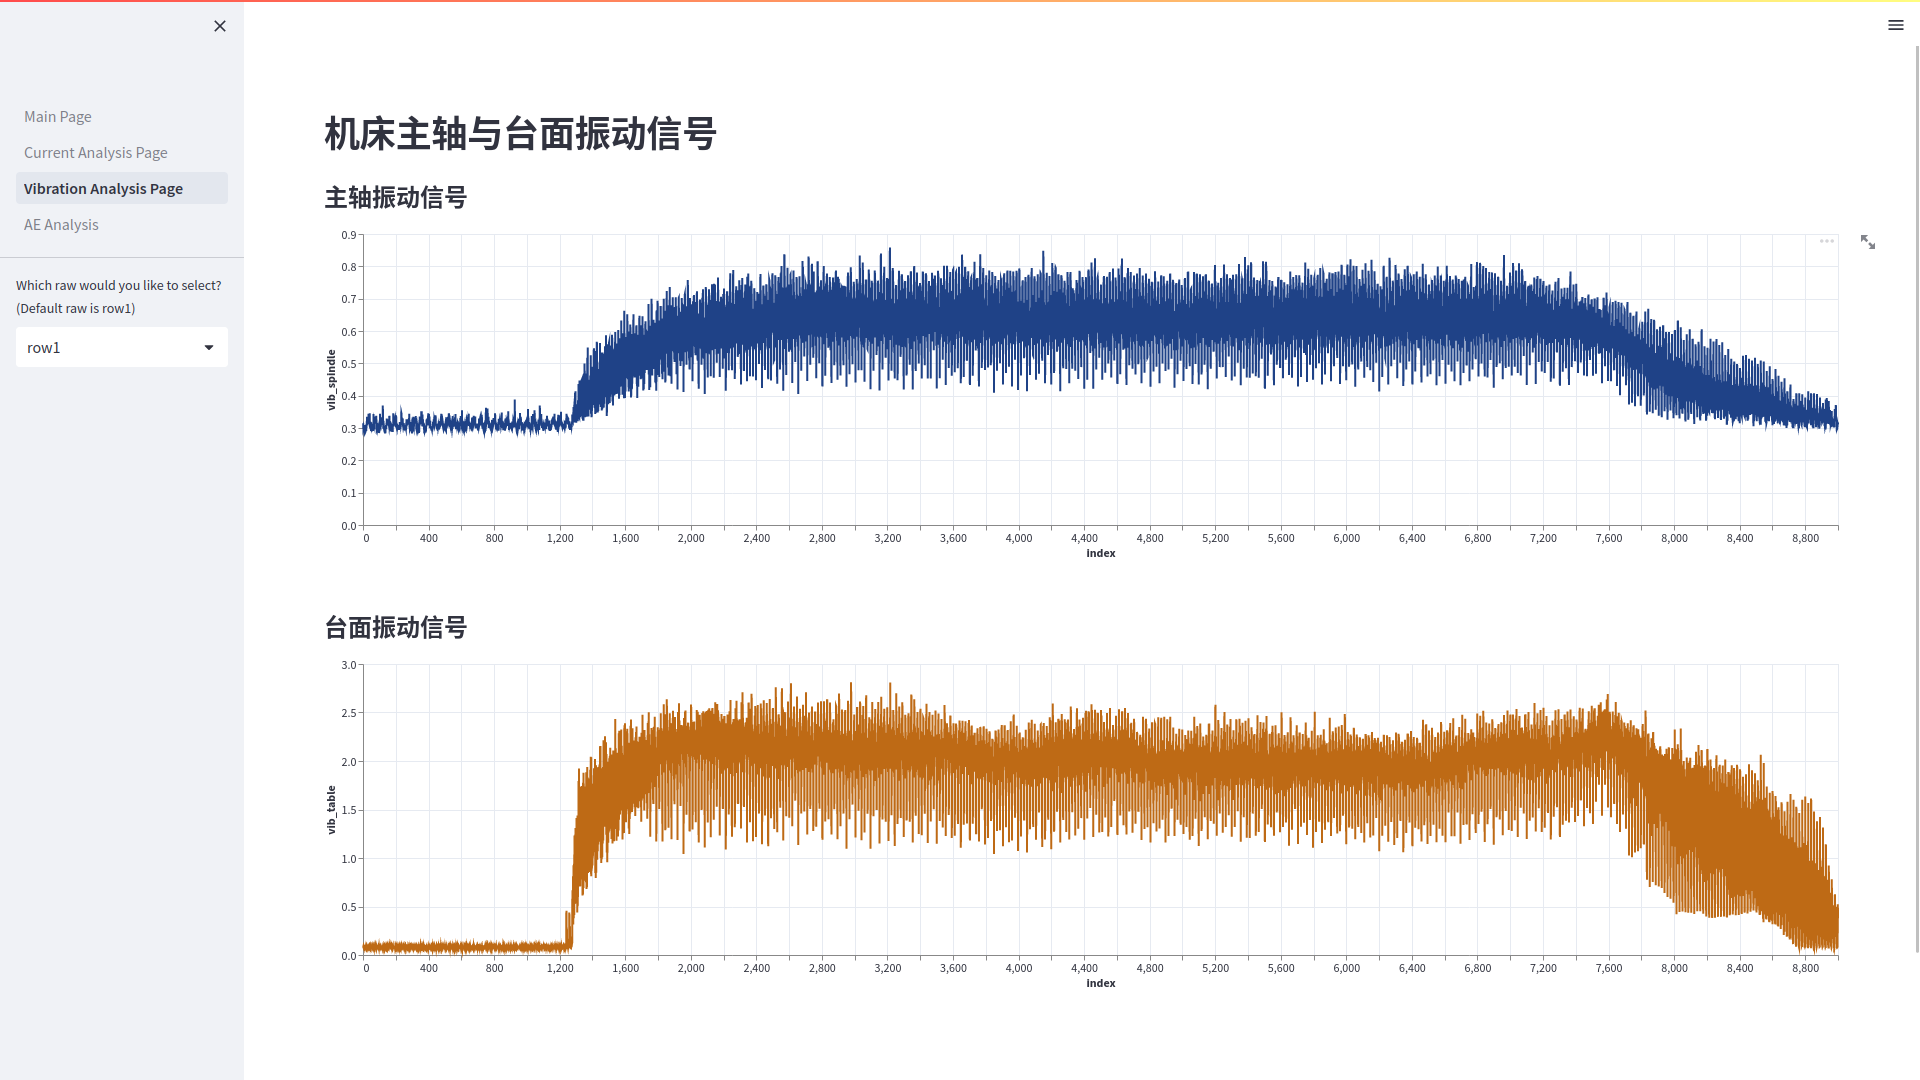
\includegraphics[width=6cm]{Chapter5/vib.jpeg}
% \label{fig_22}
\caption{振动数据分析}
\end{minipage}
\begin{minipage}[t]{0.48\textwidth}
\centering
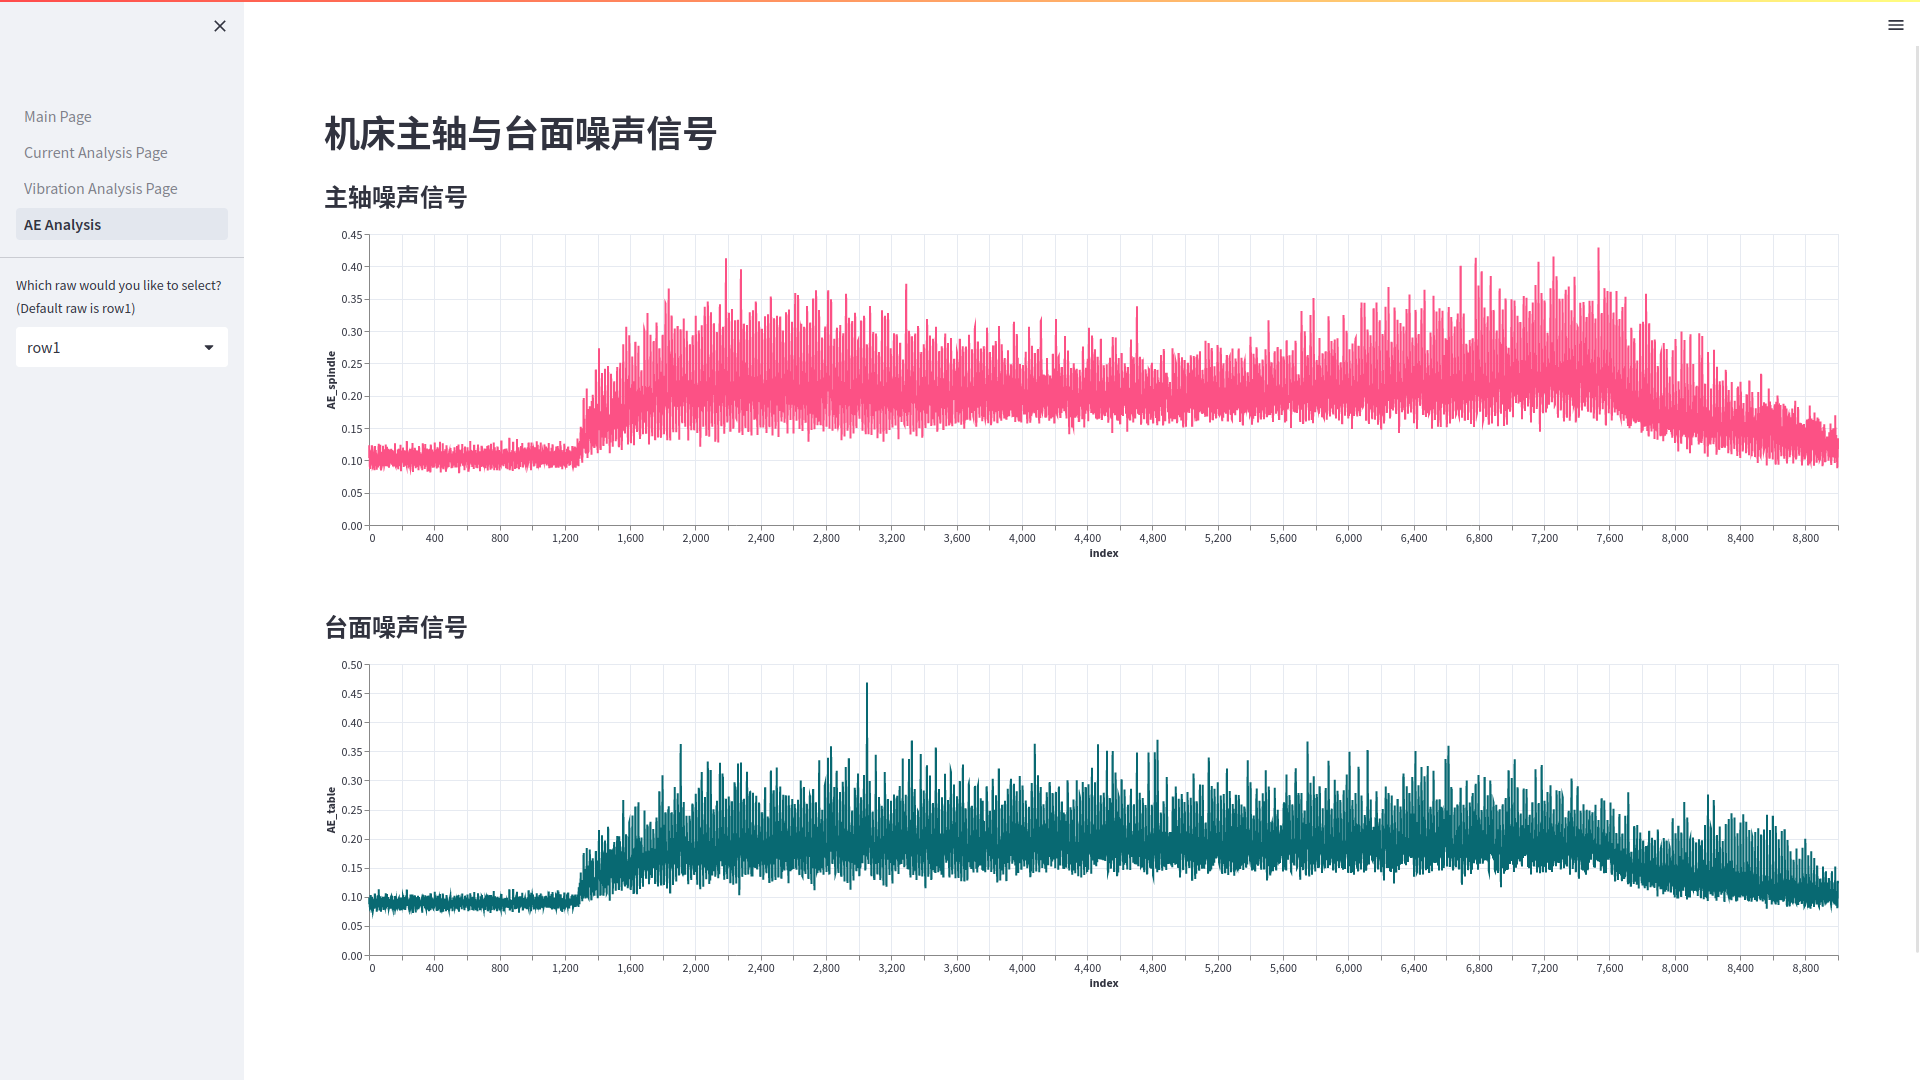
\includegraphics[width=6cm]{Chapter5/noise.jpeg}
  \caption{噪声数据分析}
% \label{fig_23}
\end{minipage}
\end{figure}
% 
